\newpage
\section{I class diagram}
\subsection{Il modello di dominio}
\begin{figure}[h!]
	\centering
	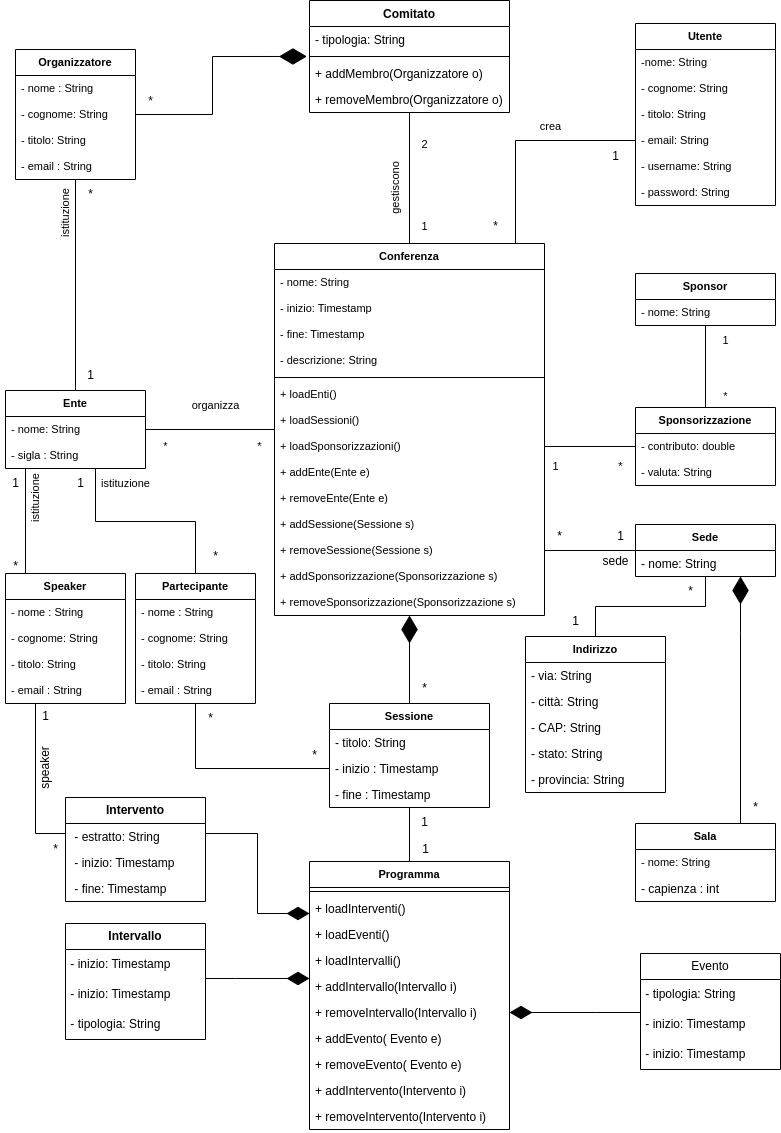
\includegraphics[scale=0.5]{Immagini/Schema_Concettuale.png}
	\caption{Class Diagram del modello di dominio}\label{uml:modellodominio}
\end{figure}

\newpage
\subsection{I controller}
\subsubsection{Controller.Create}

\begin{figure}[h!]
	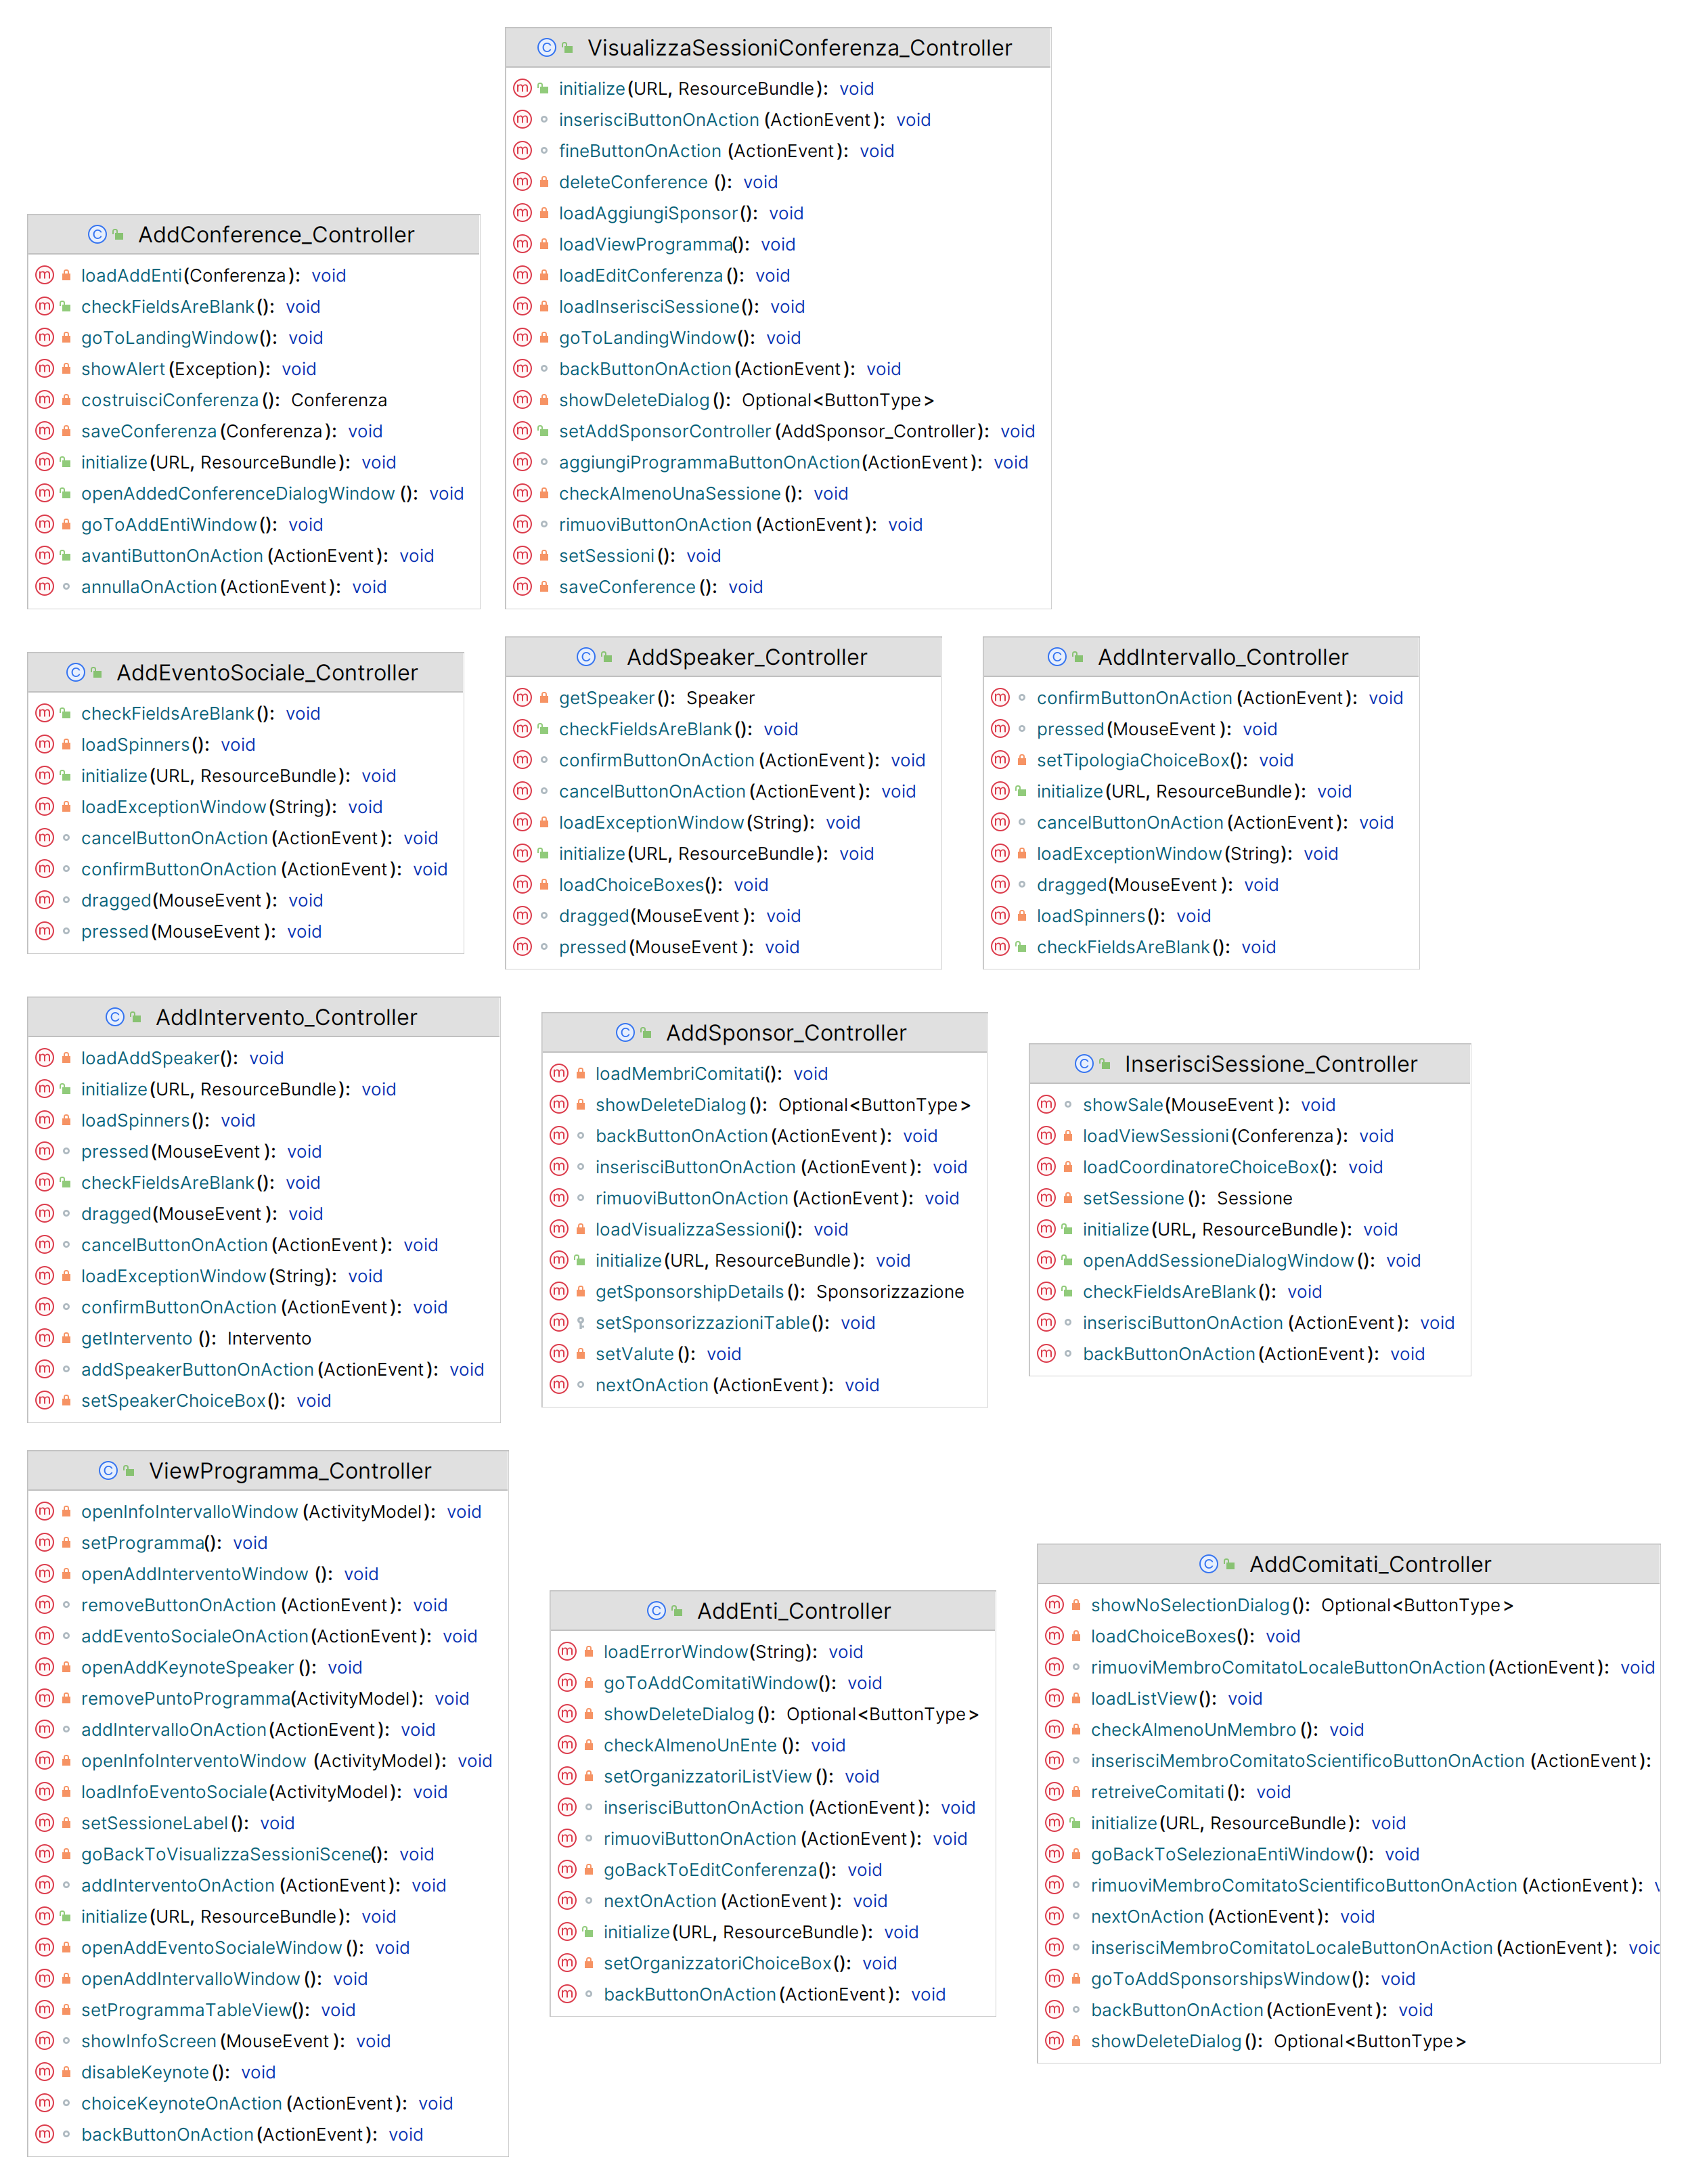
\includegraphics[scale=0.17]{Immagini/Controller_Creazione.png}
	\caption{Controller per la fase di creazione}
\end{figure}
\newpage
\subsubsection{Controller.Edit}
\begin{figure}[h!]
	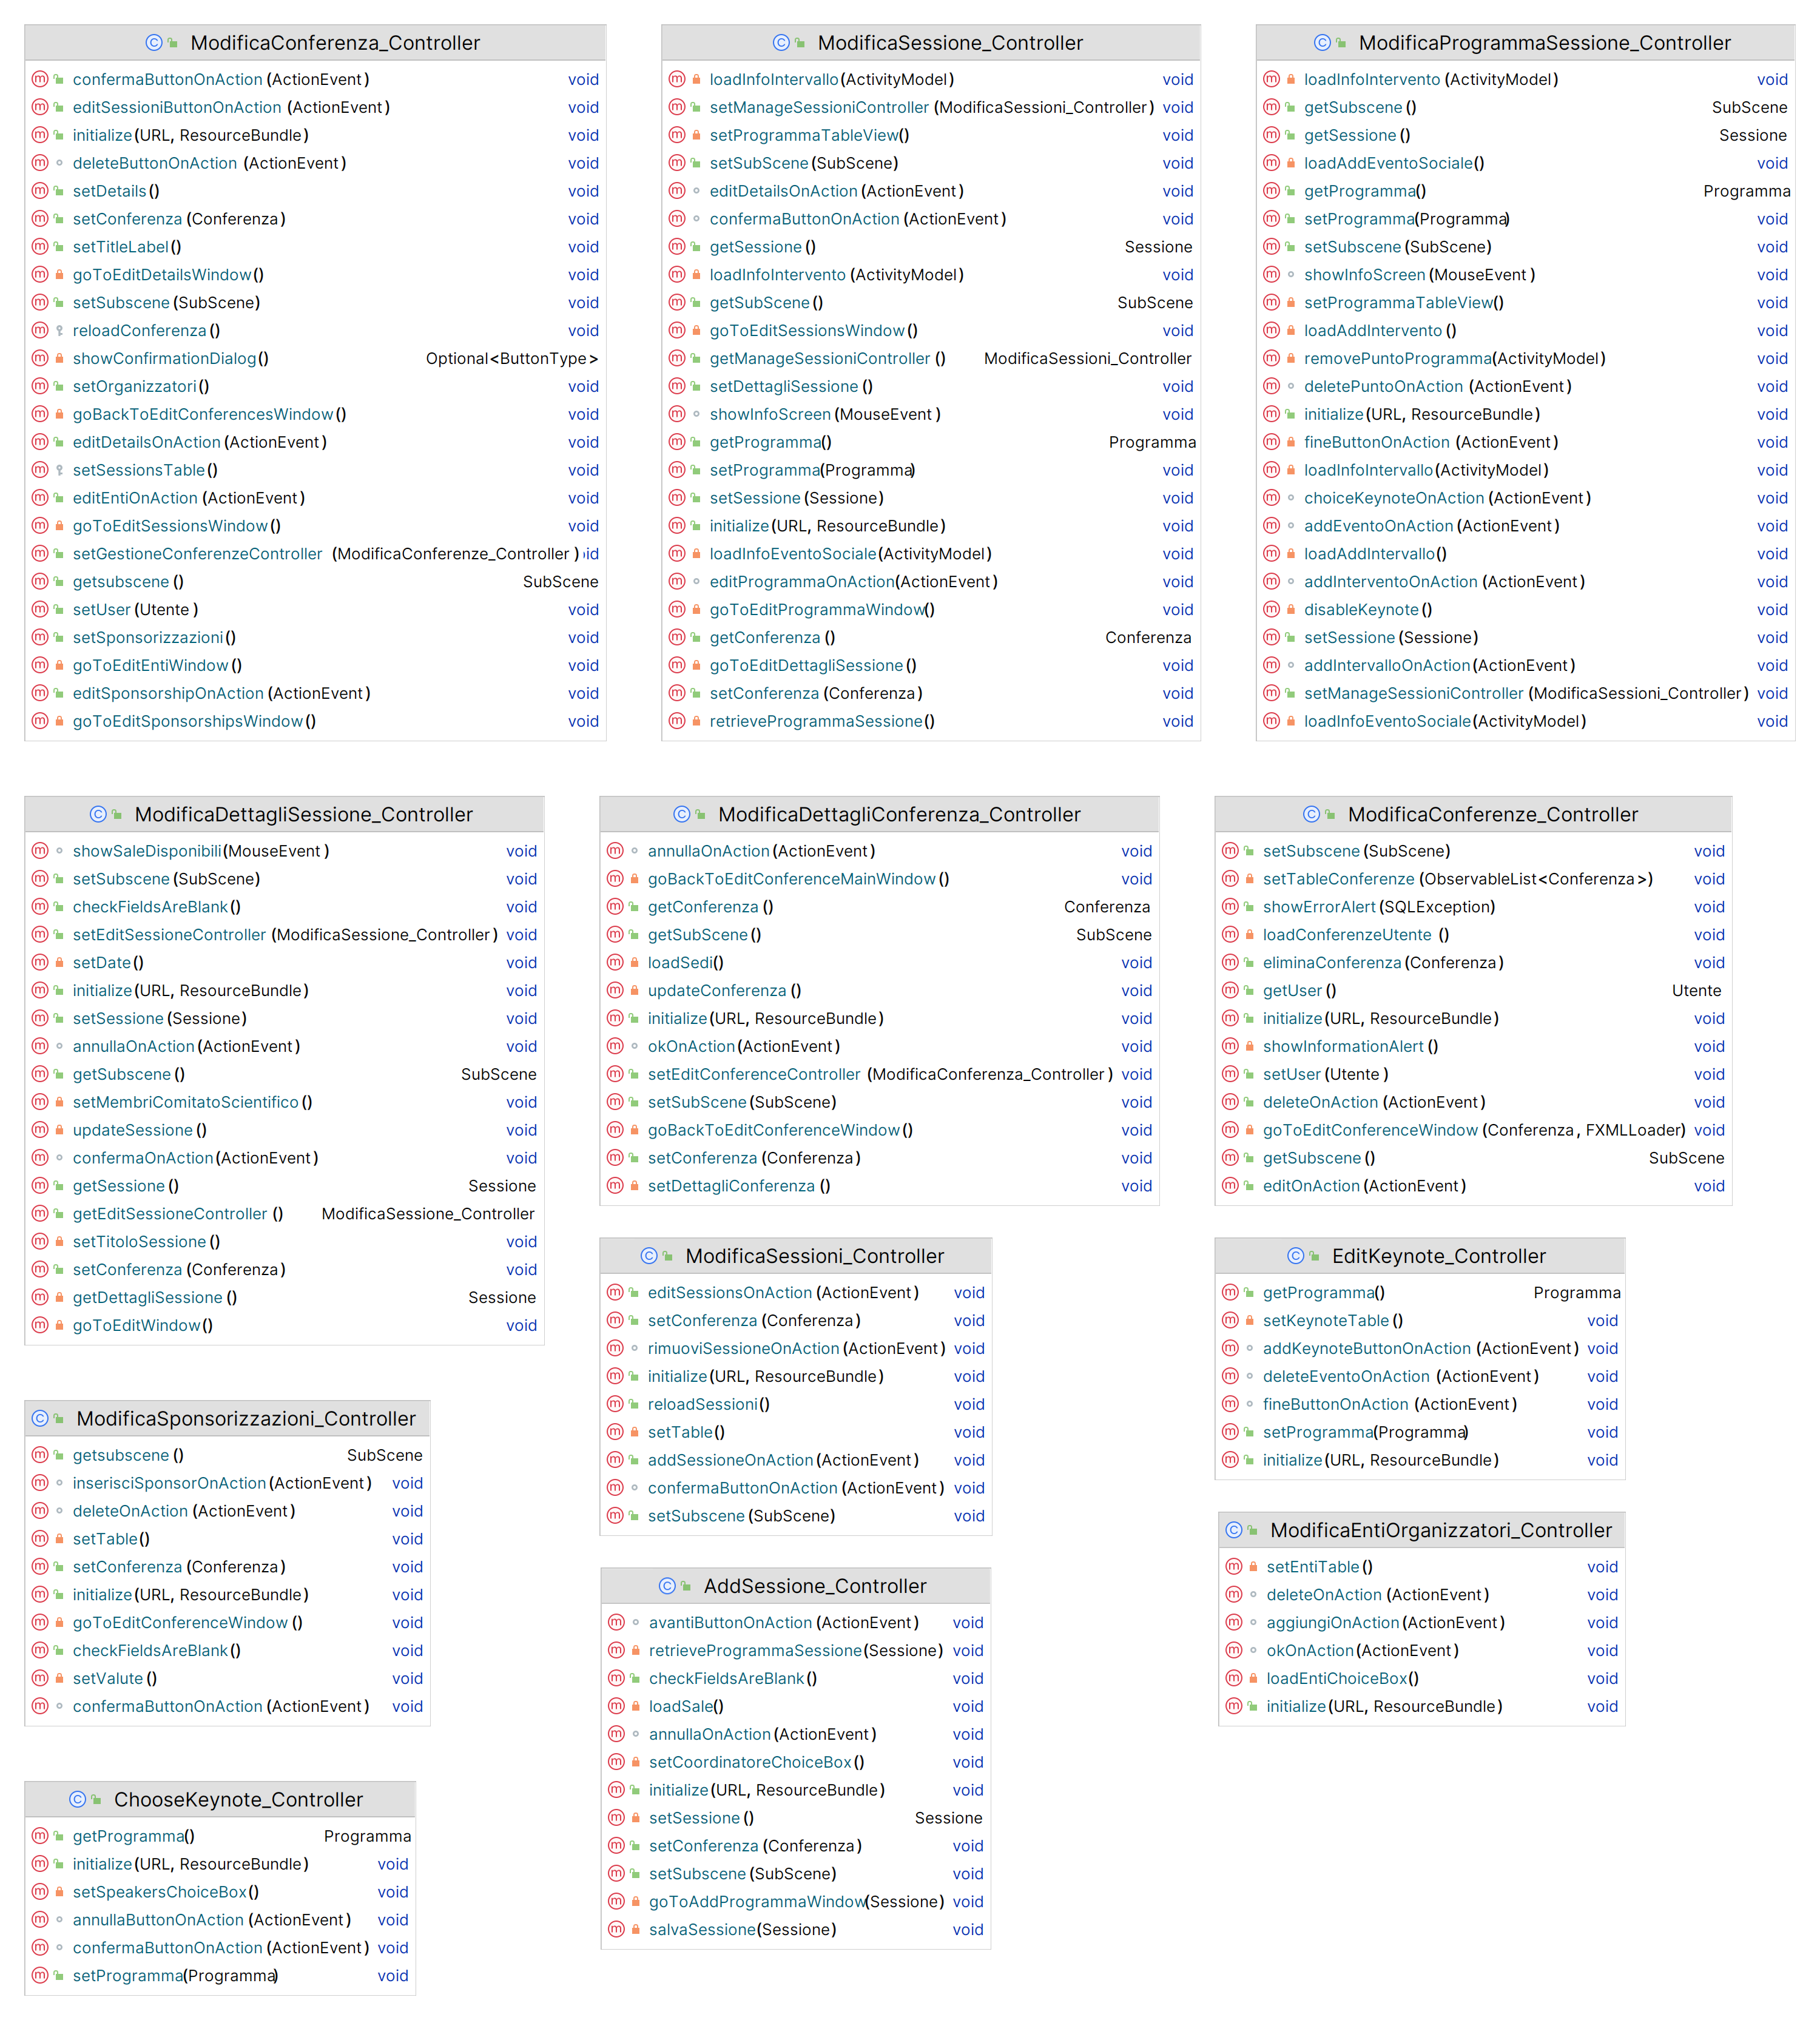
\includegraphics[scale=0.17]{Immagini/Controller_Modifica.png}
	\caption{Controller per la fase di modifica}
\end{figure}

\subsubsection{Controller.Login}
\begin{figure}[h!]
	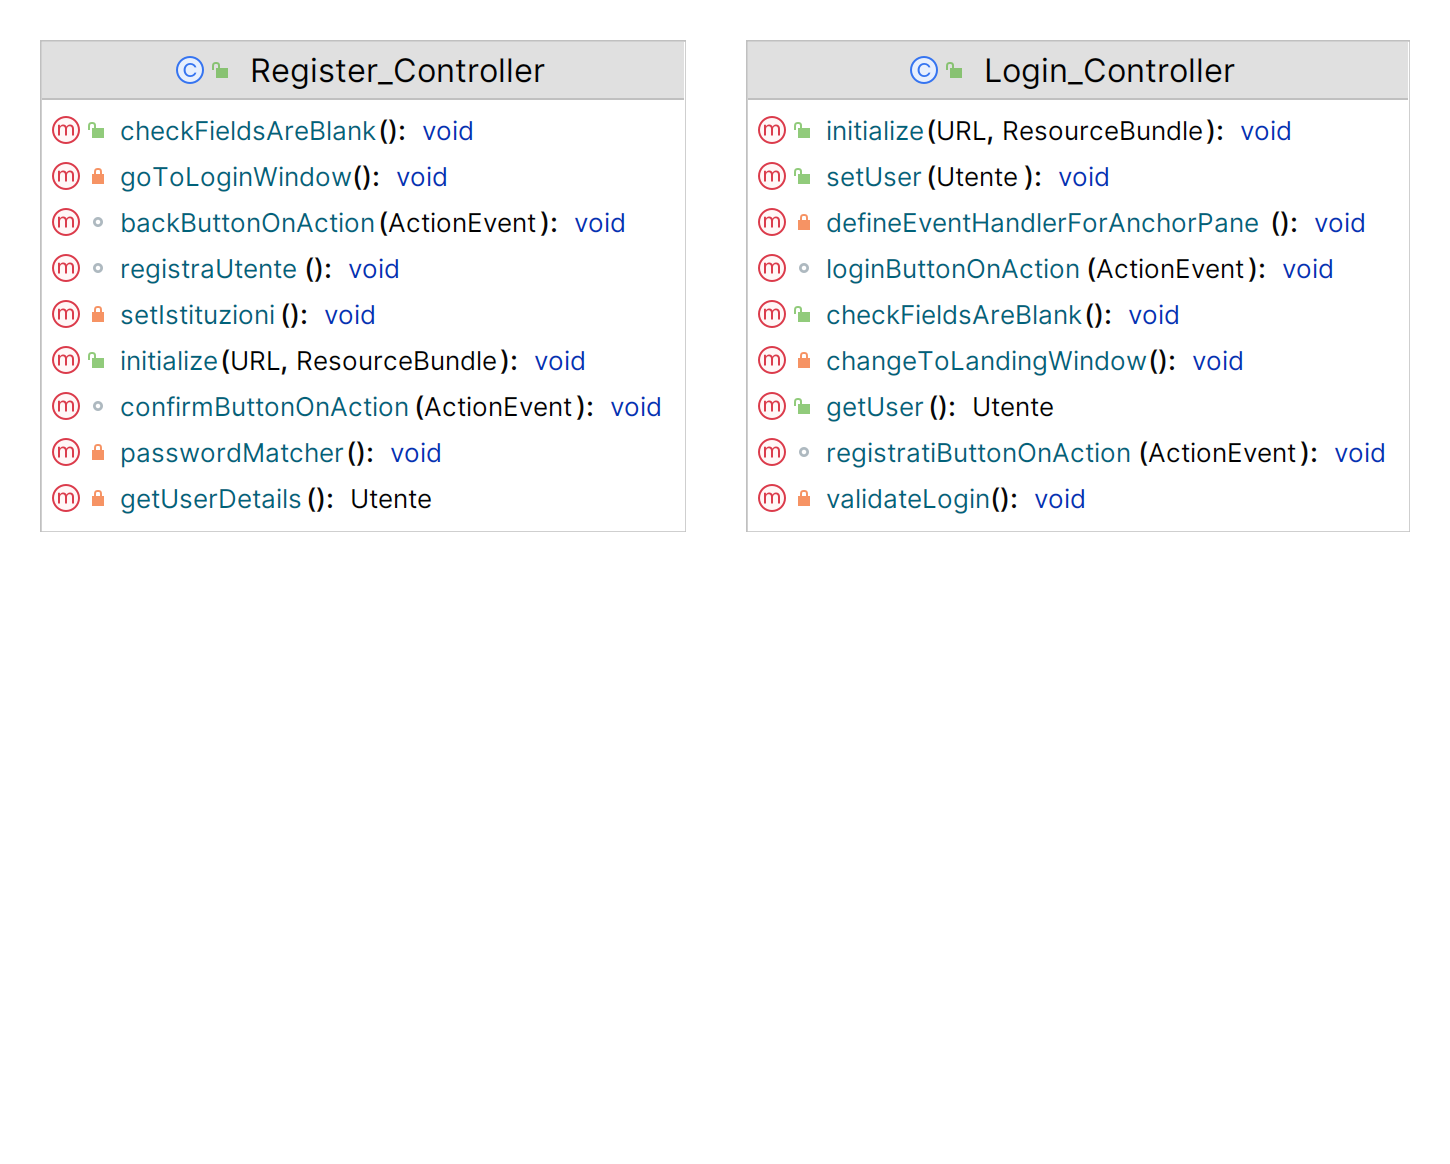
\includegraphics[scale=0.2]{Immagini/Controller_Login.png}
	\caption{Controller per la fase di login e registrazione}
\end{figure}

\subsubsection{Controller.Stats}
\begin{figure}[h!]
	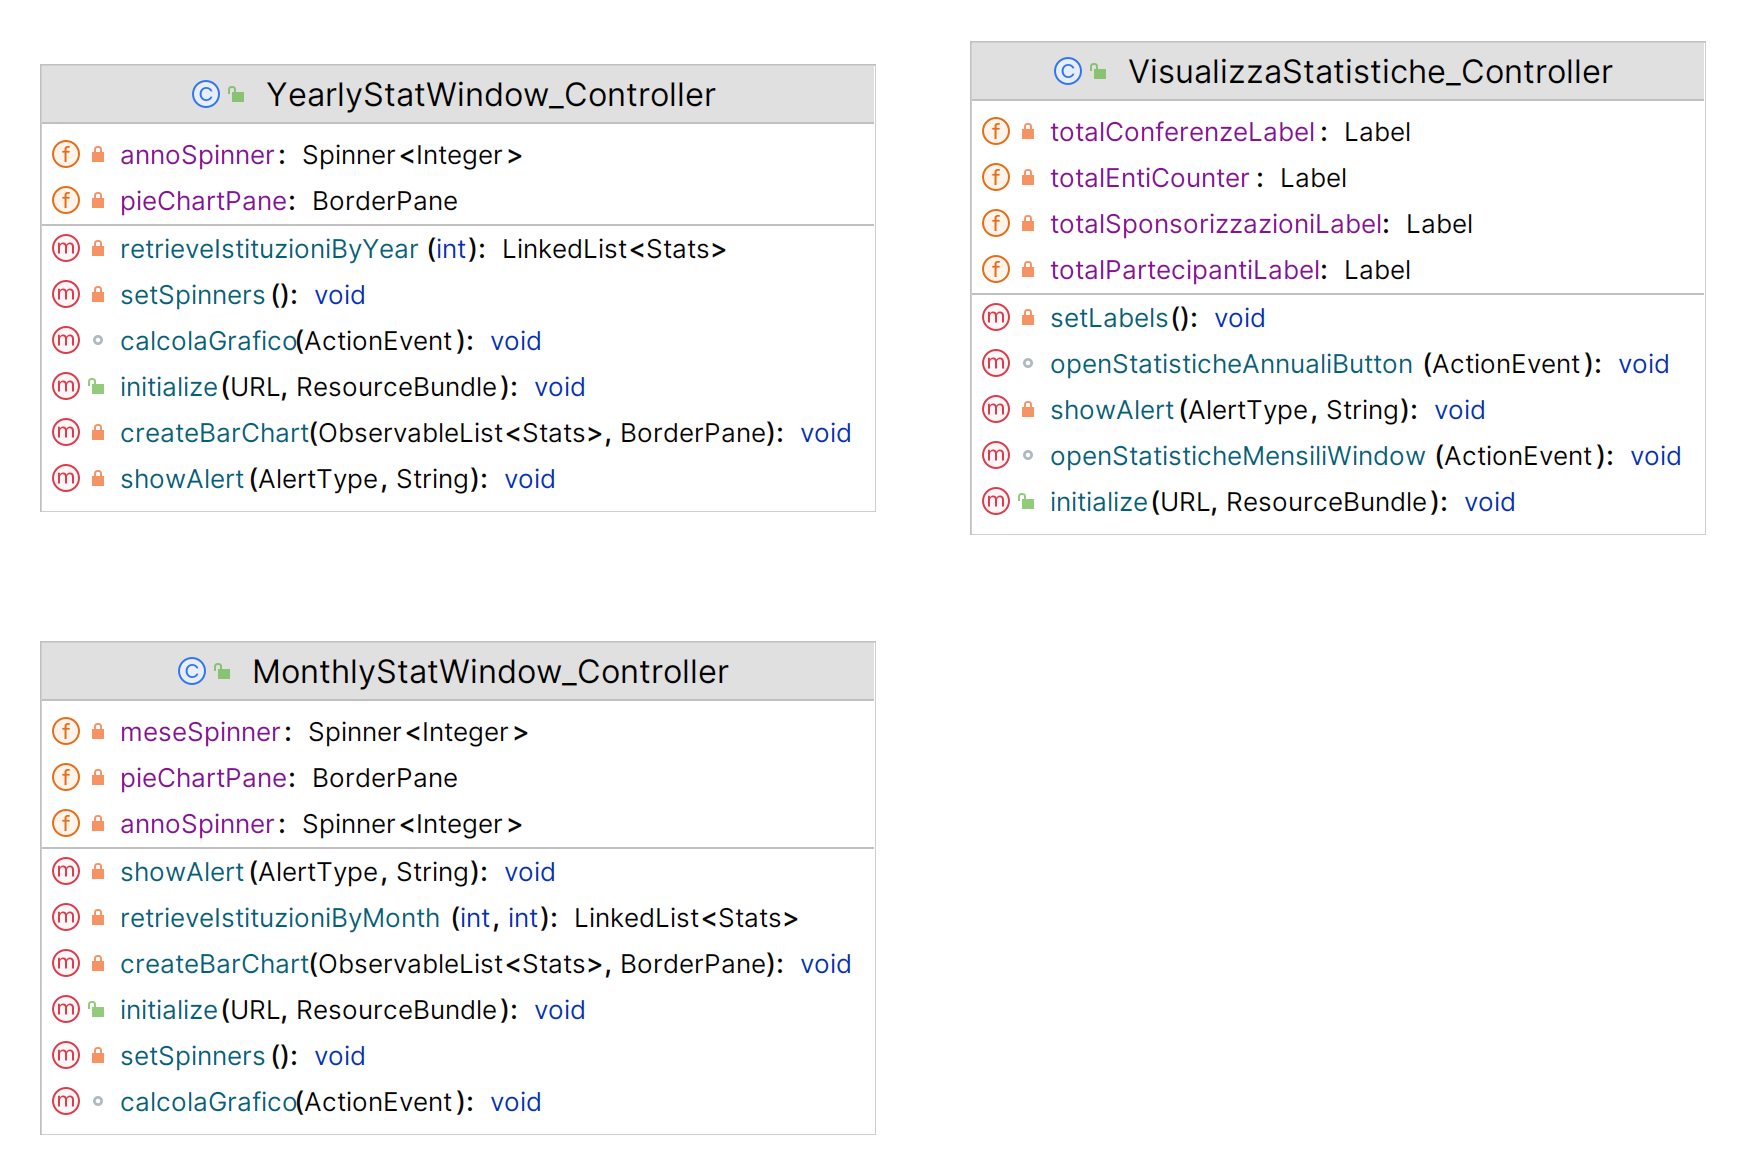
\includegraphics[scale=0.2]{Immagini/Controller_Statistiche.png}
	\caption{Controller per la fase di visualizzazione delle statistiche}
\end{figure}
\newpage
\subsubsection{Controller.View}
\begin{figure}[h!]
	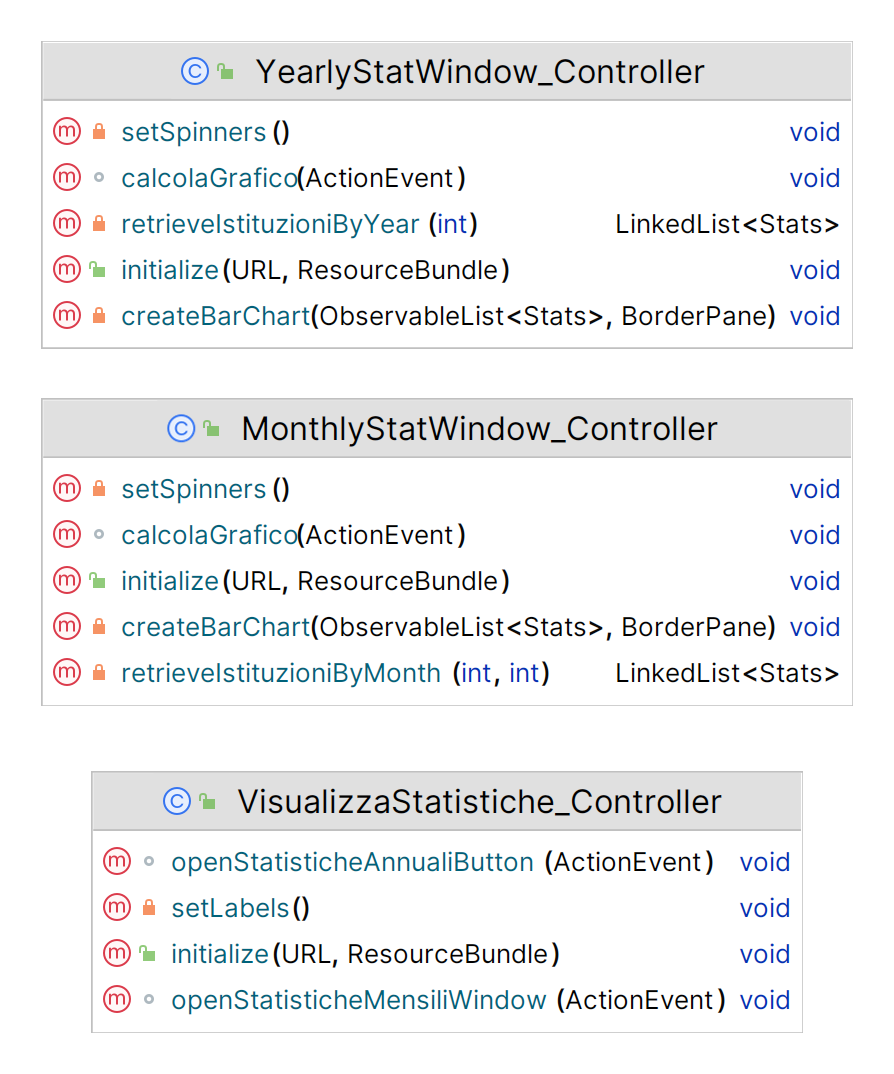
\includegraphics[scale=0.17]{Immagini/Controller_Visualizzazione.png}
	\caption{Controller per la fase di visualizzazione delle conferenze}
\end{figure}
\newpage
\subsection{Le classi DAO}
\begin{figure}[h!]
	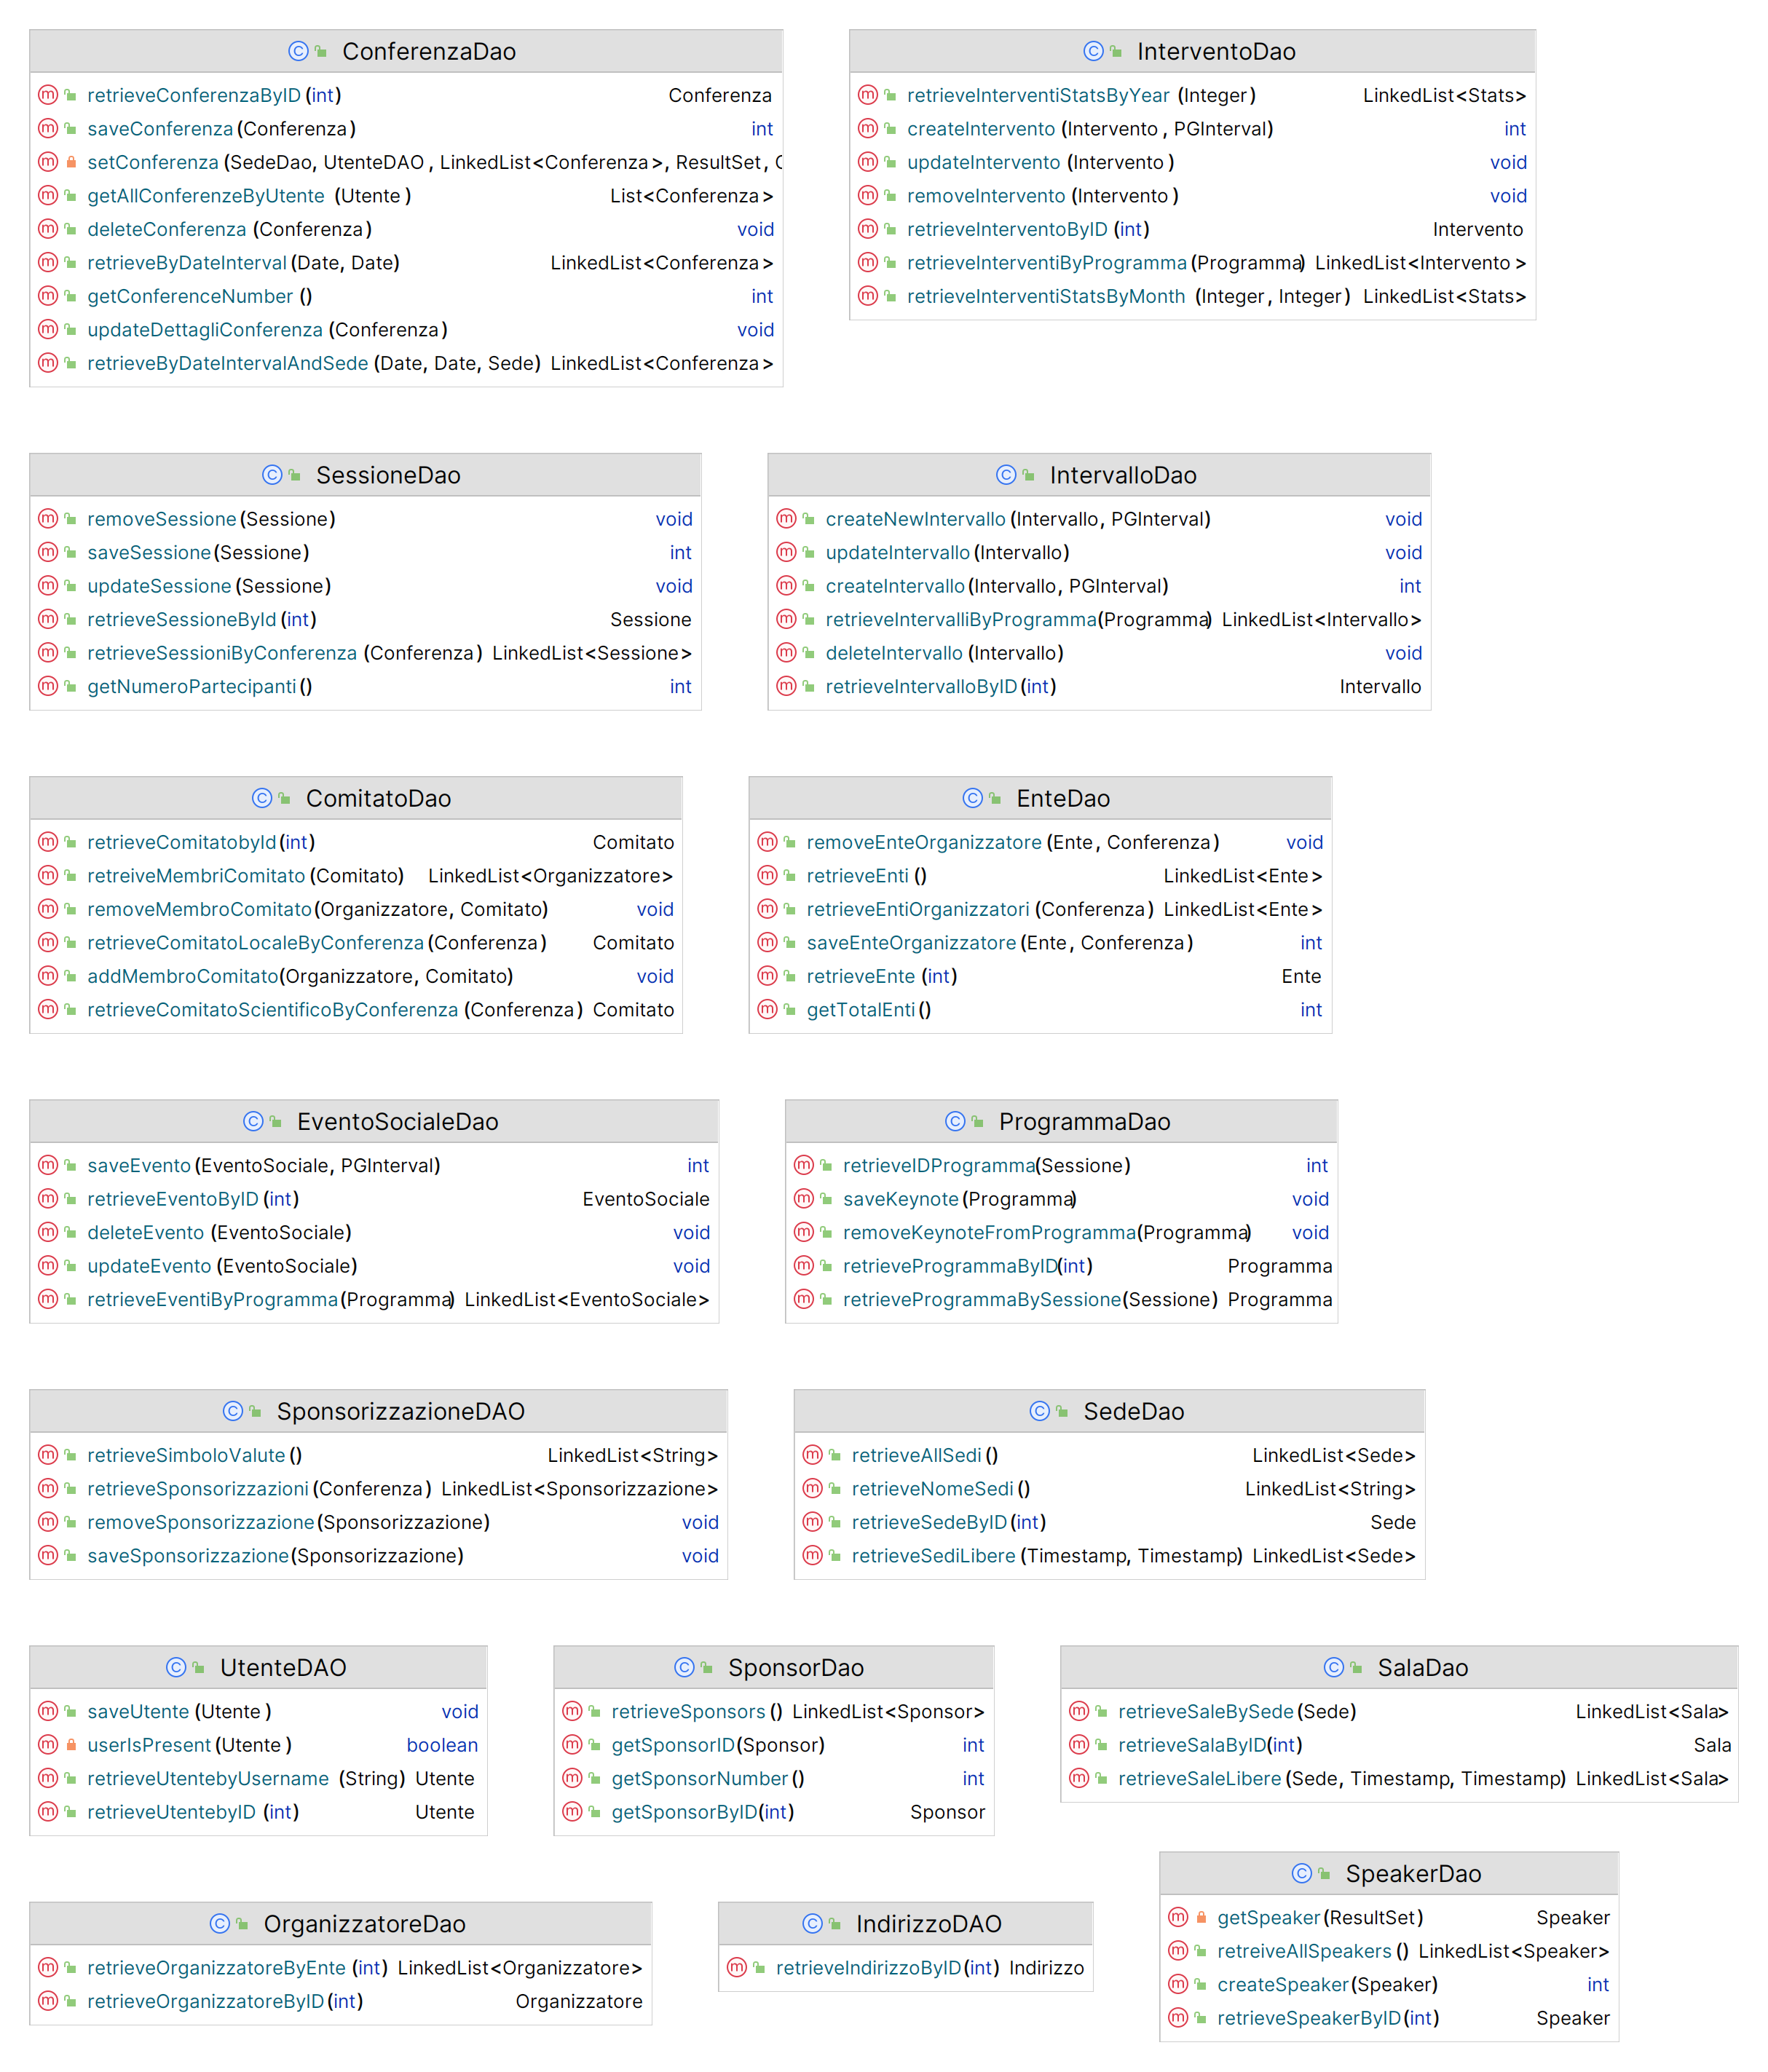
\includegraphics[scale=0.2]{Immagini/ClassiDAO.png}
	\caption{Classi DAO}
\end{figure}